\documentclass[authoryear,preprint]{sigplanconf}

\usepackage{amsmath}
\usepackage{amsfonts}
\usepackage{amssymb}
\usepackage{amsthm}
\usepackage{algorithm2e}
\usepackage{listings}
\usepackage{xcolor}
\usepackage{tikz}
\usepackage{booktabs}
\usepackage{subfigure}
\usepackage[english]{babel}
\usepackage{blindtext}
\usetikzlibrary{shapes.geometric, arrows,chains}
\bibliographystyle{abbrvnat}
\usepackage{url}
\usepackage{hyperref}

\usepackage{color}

\definecolor{dkgreen}{rgb}{0,0.6,0}
\definecolor{gray}{rgb}{0.5,0.5,0.5}
\definecolor{mauve}{rgb}{0.58,0,0.82}
\usepackage{enumitem}
\newlist{steps}{enumerate}{1}
\setlist[steps, 1]{label = Step \arabic*:}

\lstset{frame=tb,
  language=Java,
  aboveskip=3mm,
  belowskip=3mm,
  showstringspaces=false,
  columns=flexible,
  basicstyle={\small\ttfamily},
  numbers=left,
  numberstyle=\tiny\color{gray},
  keywordstyle=\color{blue},
  commentstyle=\color{dkgreen},
  stringstyle=\color{mauve},
  breaklines=true,
  breakatwhitespace=true,
  tabsize=3
}

\begin{document}

\special{papersize=a4}
\setlength{\pdfpageheight}{\paperheight}
\setlength{\pdfpagewidth}{\paperwidth}


\title{Identifying Algorithmic Complexity Vulnerabilities Caused by
Input-Dependent Nested Loops}

\authorinfo{Mujahid Masood,Rafique Nazir}{mujahid.masood@stud.tu-darmstadt.de,rafique.nazir@stud.tu-darmstadt.de}{}
\maketitle

\section{Problem Statement}
\label{sec:problemstatement}

The single-threaded event model of JavaScript makes it vulnerable
to a specific class of denial of service attack called algorithmic
complexity attacks. These attacks consist of exploiting the worst
case performance of algorithms to trigger slow computations that
block the event loop for a large period of time. The focus of this
project is to
\begin{itemize}
\item Identify the functions in code.
\item Identify the input parameters to the functions.
\item Identify the loops using input parameters of functions.
\item Impact of using function input parameters with loops in terms
of execution time as well as denial of service attack.
\end{itemize}


\section{Input dependent loops and execution time}
\label{sec:introduction}
Execution time of the functions is really important to write scalable applications. In normal application overall execution time of function depend on the slowest function.

Consider the code in Listing \ref{l:iterate} we have iterate function which has max as input parameter, it has one loop which is iterating up till max.

So caller of function can pass input of \begin{math} 10_{10} \end{math} and execution time of simple function with 1 loop will be around \textit{11s}.

\begin{lstlisting}[caption=iterate function with 1 loop,label=l:iterate,language=Java]

function iterate(max){

    var start = process.hrtime();
    var precision = 3;
    for(var i = 0; i< max; i++){
        var c = 10 + 5;
    }

    var elapsed = process.hrtime(start)[1] / 1000000;
    
	console.log(
		process.hrtime(start)[0] + " s, "+
		elapsed.toFixed(precision)+" ms - " 
	);
}

\end{lstlisting}

If other functions in application are taking less time, iterate
function is subject to performance bug and also security bug specially
in node modules.

This problems gets interesting if we introduce nested loops
i.e, 2 or 3 nested loops. Consider the code in Listing 2. Function
double loop has input parameters max and 2 nested loops. Client
of doubleLoop can pass input max 105
and can introduce as delay
of around 6 s, 491.041 ms . Important thing to note is function is
only doing simple sum of 10 and 5 but due to input dependent loop
execution time of function takes much time.

\begin{lstlisting}[caption=doubleLoop function with 2 nested loop,label=l:doubleLoop,language=Java]

function doubleLoop(max){

    var start = process.hrtime();
    var precision = 3;
    for(var i = 0; i< max; i++){
    	for(var j=0; j< i; j++){
			 var c = 10 + 5;
 		}
 	}

    var elapsed = process.hrtime(start)[1] / 1000000;
	console.log(
		process.hrtime(start)[0] + " s, "+
		elapsed.toFixed(precision)+" ms - " 
	);
}

doubleLoop(Math.pow(10,5));

\end{lstlisting}

As we increase the nested loops input to the parameter gets
smaller. A function with 3 nested loops and input parameter max
can have execution time of around 6 s with max = 103.2
Consider the code in Listing 3.

\begin{lstlisting}[caption=tripleLoop function with 2 nested loop,label=l:tripleLoop,language=Java]

function tripleLoop(max){

    var start = process.hrtime();
    var precision = 3;
    for(var i = 0; i< max; i++){
    	for(var j=0; j< i; j++){
    		for(var k=0; k< max; k++){
				 var c = 10 + 5;
 			}
 		}
 	}

    var elapsed = process.hrtime(start)[1] / 1000000;
	console.log(
		process.hrtime(start)[0] + " s, "+
		elapsed.toFixed(precision)+" ms - " 
	);
}

tripleLoop(Math.pow(10,3.2));

\end{lstlisting}


\section{Problems with using loops depending on function input parameters}
\label{sec:problems}
Code in Listing \ref{l:doubleLoop} and Listing \ref{l:tripleLoop} are not only subject to performance issues but also to denial of service (DoS) attacks. Attacker can control the input parameter and can introduce delay of 10-15 seconds in the execution time of function. Node.js security experts consider any slowdown larger than one second as security relevant.

\section{Avoiding the problem}
\label{sec:avoiding}

Following are some approaches which can be used to avoid the problem with input dependent nested loops.

\subsection{Approach 1 : Introduce Upper bound on input parameters}
One simple way to avoid such problem is introducing upper bound on input parameter.
Consider the code in Listing \ref{l:avoidProblem} which exits from the function if input exceeds the given bound which is \begin{math} 10^{2} \end{math}.

\begin{lstlisting}[caption=avoidProblem function with 3 nested loop,label=l:avoidProblem,language=Java]

function avoidProblem(max){
	if(max > Math.pow(10,2)) {
		return;	
	}
    for(var i = 0; i< max; i++){
    	for(var j=0; j< i; j++){
    		for(var k=0; k< max; k++){
				 var c = 10 + 5;
 			}
 		}
 	}
}

avoidProblem(Math.pow(10,3.2));

\end{lstlisting}

\subsubsection{Problems with Approach 1}

Introducing such input bound checks as in Listing \ref{l:avoidProblem} requires full understanding of the code and also the usage of function.

\subsection{Approach 2 : Changing the logic} 
Other way can be changing the logic from nested loops to maybe introducing new functions which means one needs to find places where input dependent functions with loops are used in the code.
\subsubsection{Problems with Approach 2}
\begin{itemize}
\item Code is already deployed in production environment.
\item JavaScript uses minified versions of files.
\item JavaScript file can have 10000s lines of code.
\item Different variations of functions.
		\begin{itemize}
			\item JavaScript can use assignment of function to other variable 
				e.g, var a = function() {}
			\item Using anonymous functions
				e.g, (function())
			\item JavaScript also uses nested functions
				e.g, (function(a, function(){}))
		\end{itemize}
\item Different variations of Loops
	 e.g  For, While, For In, forEach etc.
\item Assignment of function input parameter to other variables and using that in loop.
\item Using input parameter in function call which in turn uses for loop.
	 
			
\end{itemize}

\section{Our Approach}
\subsection{High Level Steps}
\begin{itemize}
	\item Statically analyse JavaScript code.
	\item Find out if code uses function.
	\item Find out if function uses input parameters.
	\item Find out if function uses loops.
	\item Find out if loops use input parameters directly or indirectly.
	\item Write vulnerable output.
	\item Manually validate the results.
			\begin{itemize}
				\item Manually trigger the identified function.
				\item Calculate the execution time of function on different inputs
			\end{itemize}
\end{itemize}

\subsection{Implementation Technologies}
\begin{itemize}
	\item Static Analyser : Google Closure Compiler for static analysis.
	\item Programming Language : Java 8
	\item Build tool : Maven
	\item Bash Script (Utility)
			\begin{itemize}
				\item clone.sh : cloning git code to specified directory
				\item search.sh: Bash script to search JavaScript Projects on Github, opens the browser session for displaying results.\end{itemize}
\end{itemize}


\subsection{Detailed Steps}

\begin{figure}[ht]
\centering
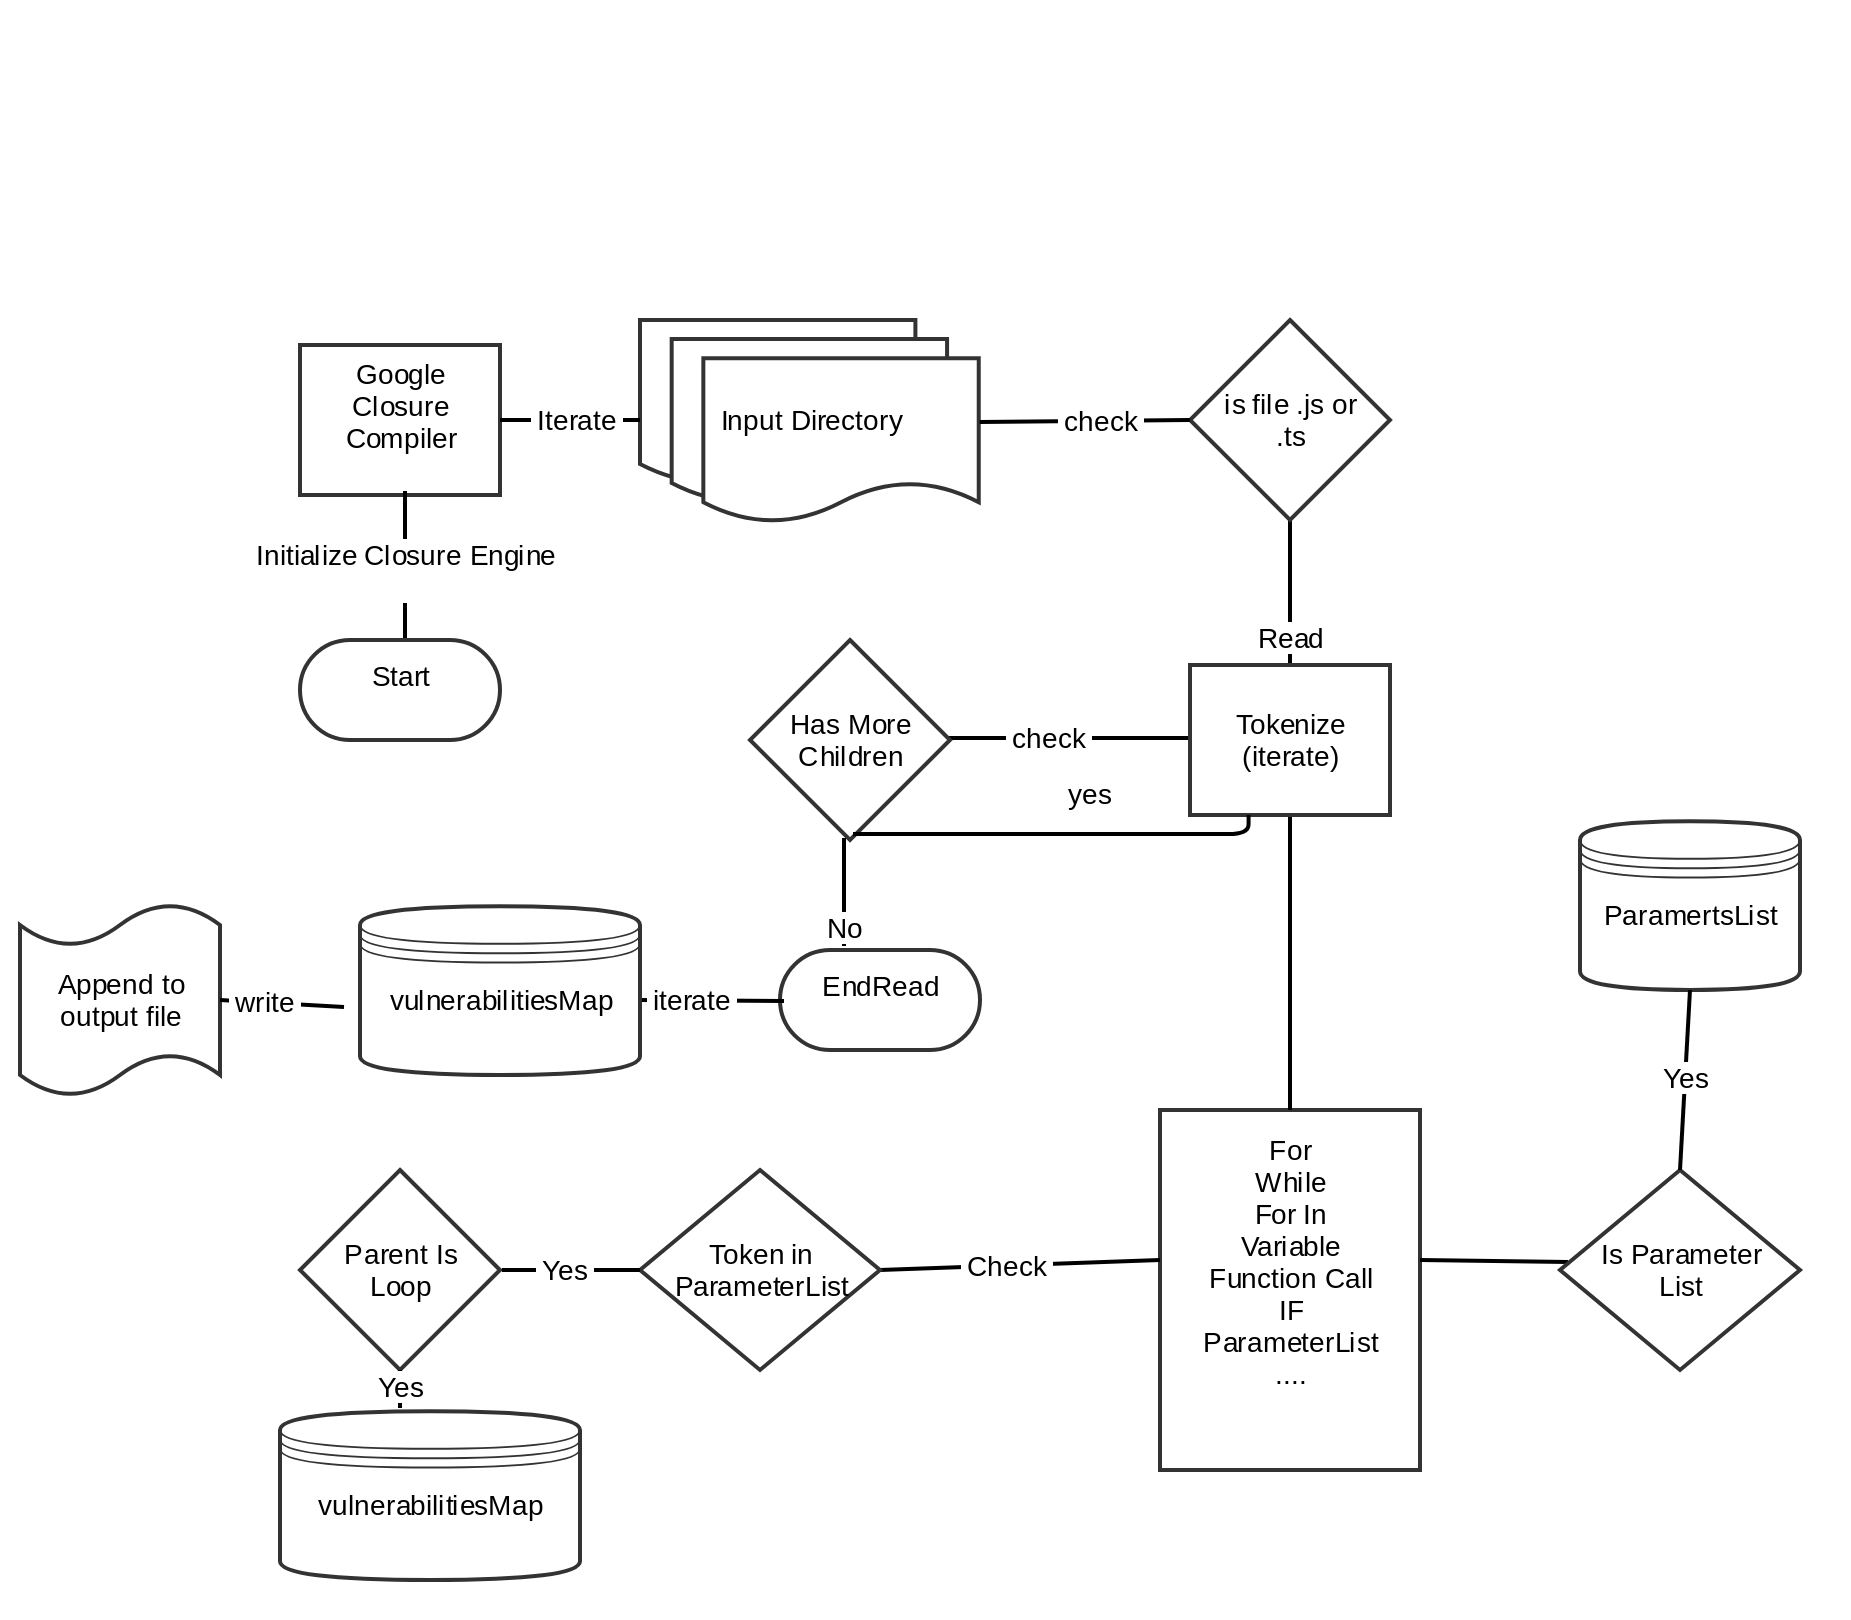
\includegraphics[width=1\linewidth]{figures/workflow}
\caption[Implementation Detail]{\label{f:workflow}Implementation Detail.}
\end{figure}

\begin{itemize}
\item Iterate through the directory.
\item Check for any .js or .ts file.
\item Initialize Google Closure Engine.
\item Read the JavaScript File.
\item Tokenize the JavaScript code.
\item Iterate through the tokens.
\item Check if the token is function, save the reference for future use.
\item Check if token is the parameter list, add it in parameter list.
\item Check if the variable is present in parameter list.
\item Check if the parent of variable is loop.
\item If variable is loop and present in parameters, add it into vulnerabilitiesMap.
\item At the end of all tokens print the output in text file.
\end{itemize}

\subsection{Project Structure}

\begin{figure}[ht]
\centering
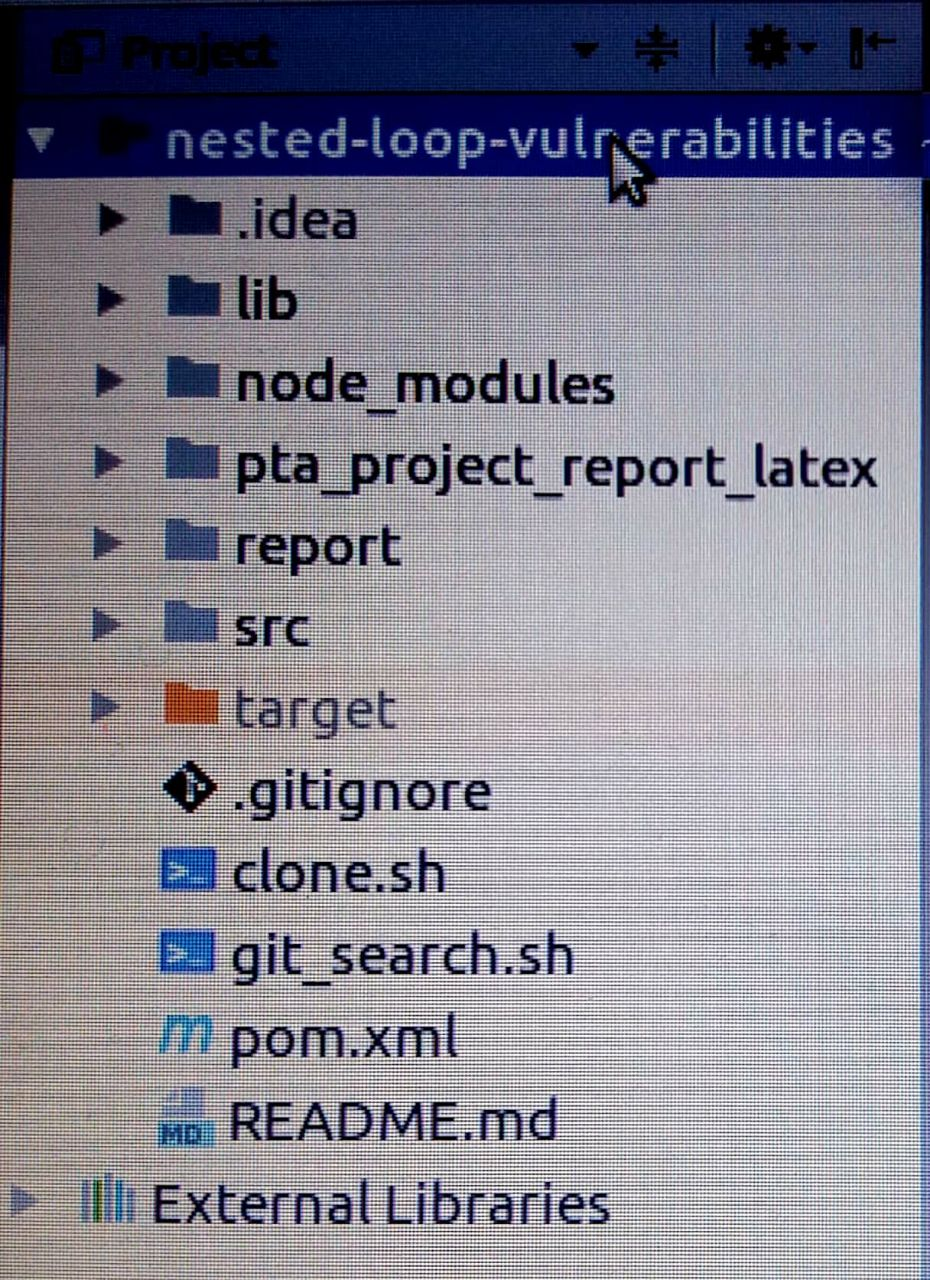
\includegraphics[width=1\linewidth]{figures/structure}
\caption[Project Structure]{\label{f:structure}Project Structure.}
\end{figure}

\begin{itemize}
\item lib : This folder contains libraries.
\item node modules : This folder contains the npm modules on which we have run the analyis.
\item report : Contains the project report.
\item src : Contains the source classes (Java Classes), actual code with implemented logic.
	\begin{itemize}
		\item main
			\begin{itemize}
		\item AnalyzerClient : Main class to invoke the analyser.
		\item ClosureEngine : Class for Google closure related settings, mainly initializes the Google Closure Compiler.
		\item OutputWriter : Class to write the output vulnerabilities in text file.
		\item StaticAnalyzer : Class has main logic, iterates the JavaScript code, checks for functions, loops and decides vulnerabilities.\end{itemize}
		
		\item test
			\begin{itemize}
				\item resources : Contains our test cases and output files
			\end{itemize}
		
	\end{itemize}

\item .gitignore : Contains git ignored files.
\item clone.sh : Bash script to clone the git directory to specified location.
	\begin{itemize}
		\item It takes two input parameters git clone directory and location where to clone the project for example to run the file.
		sh clone.sh https://github.com/project.git /nested-loop-vulnerabilities/node modules
		
		It will create new folder named project.git under node modules directory and clone the project in it.
		
	\end{itemize}

\item search.sh : Searches the JavaScript projects on github, to show the results it opens google chrome browser.

\item pom.xml : It contains maven related configurations.
\item README.md : Contains the instructions on how to use project.
		
\end{itemize}

\section{Results}
Following section discusses the results on our own test cases and also on node modules.
In Project code index.js under resources folder contains our test cases, we will demonstrate a few from index.js file.

\subsection{Manual Tests}
\begin{figure}[ht]
\centering
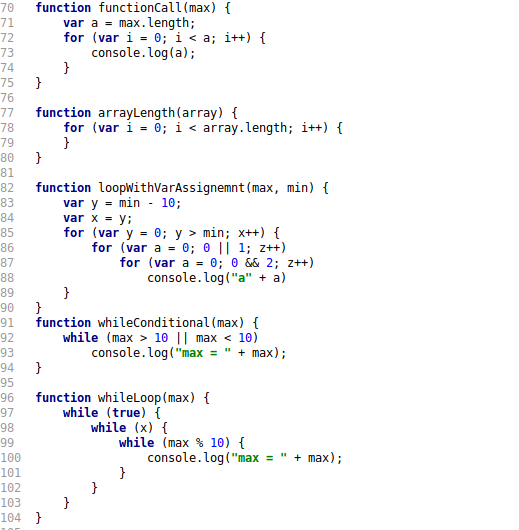
\includegraphics[width=1\linewidth]{figures/testcases}
\caption[Manual Tests]{\label{f:testcases}Manual Tests.}
\end{figure}

From the figure \ref{f:testcases} we expect to find vulnerabilities on lines 72,78, 85, 92 and 99 because the functions use input dependent loops.
We ran the tests using our code and output is as below.

\begin{figure}[ht]
\centering
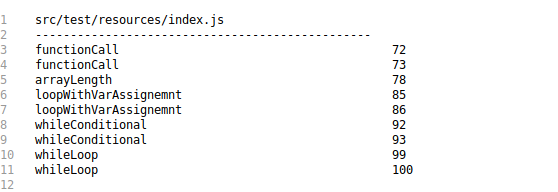
\includegraphics[width=1\linewidth]{figures/output}
\caption[Output of Manual Tests]{\label{f:testcases}Output of Manual Tests.}
\end{figure}

As we can see our code correctly identifies the specified lines where possible vulnerabilities can occur along with some false positives.
Output format is
\begin{itemize}
\item First line is file name for which analysis is done.
\item Multiple dashes for separation.
\item Subsequent lines shows function name in left column and line number in right column. In case of anonymous function output function on left is null.

\end{itemize}

\subsubsection{Validation of claim}
With above functions validation is easy we added execution time to validate our claim as shown in Listing \ref{l:doubleLoop}, \ref{l:tripleLoop}

\section{Analysing Node modules}
We run our analysis on following node modules. In order to identify nested loops we mainly focused on video streaming,audio streaming, matrix and data structure libraries to find the code using nested loops.

\begin{itemize}
\item dashjs : Library to quality framework for building video and audio players that play back MPEG-DASH content using client-side JavaScript.

\item loaddash : A modern JavaScript utility library delivering modularity, performance & extras.
\item lru cache : This is an LRU (least recently used) cache implementation in JavaScript.
\item 
\item 
\item 
\end{itemize}
We have written generalize code which can iterate on the directories and identify the


\citep{Aho86-Compilers}
\bibliography{references}

\end{document}